% !TeX spellcheck = de_DE
\chapter{Theoretische Grundlagen}
\label{sec:theorie}
Als schon im Abschnitt "Einleitung" erwähnt wurde, bei der Aufgabestellung es um eine Entwicklung einer Webanwendung geht. Die zu realisierende Software basiert sich, wie die meisten Webanwendungen, auf einer Client-Server-Architektur, wobei der Client Informationen eingibt, während der Server die eingegebene Daten empfängt, bearbeitet und speichert. 

\section{Raspberry Pi Board und Betriebsystem }
\label{sec:theorie:raspberry}
\begin{wrapfigure}{l}{0.45\textwidth}
	\fbox{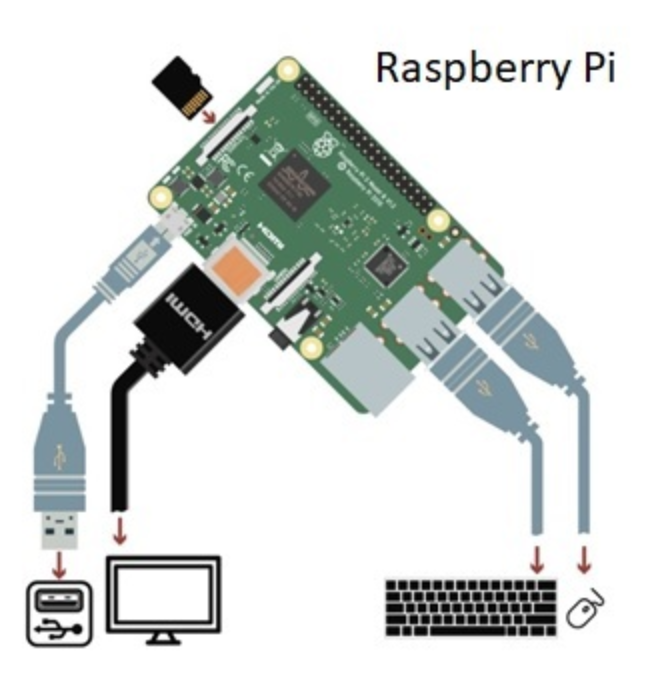
\includegraphics[width=0.42\textwidth]{gfx/rasp.png}}
	\caption{Peripherieanschlüsse des Mikrocomputers}
	\label{fig:rasp}
\end{wrapfigure}
Raspberry Pi ist ein Einplatinencomputer, wobei die verschiedene Teile des Computers, die sich normalerweise auf separaten Platinen befinden, werden hier nur auf einer dargestellt. Wie die meisten Einplatinencomputer ist der Raspberry Pi so klein wie eine Kreditkarte. Der Raspberry Pi ist eine kostengünstige Plattform - sein empfohlener Verkaufspreis beträgt weniger als 50€. Ein Mikrocomputer verfügt über alle Funktionen eines Personal Computer (PC): Prozessor, Speicher, Betriebssystem, Anschluss an einen Monitor (TV), die Vernetzung. Der Raspberry Pi verfügt im Gegensatz zu einem PC über zusätzliche Peripheriegeräte wie GPIO-Ports (General Purpose Input / Output). Über diese Pins kann der Mikrocomputer mit der elektronischen Welt der Sensoren, Bildschirmen und Aktoren interagieren. In Abbildung \ref{fig:rasp}\cite{website:3} sind die Anschlüsse schematisch dargestellt.

Für die Entwicklung der Abschlussarbeit und die Verwendung im Labor wird Raspberry Pi 3 Model B+ benutzt, an dem der RFID Leser angeschlossen wird. Das Modell "Raspberry Pi 3 B" ist eine kontinuierliche Weiterentwicklung zum Vorgängermodell "Raspberry Pi 2 B".
Der Raspberry Pi 3 enthält einen Quad-Core-Prozessor mit 1,2 GHz von Broadcom und einen SDRAM-Arbeitsspeicher mit 1 GByte.  Auf der Unterseite des Raspberry Pi befindet sich einen weiteren Chip, der wie ein kleines schwarzes Plastikquadrat aussieht. Dies ist der Direktzugriffsspeicher (RAM) des Mikrocomputers. Wenn am Pi gearbeitet wird, wird die laufende Arbeit auf dem RAM gespeichert. Nur wenn die Daten explizit auf die microSD-Karte geschrieben werden, dann werden sie zum nächsten Verwendung gespeichert und nach dem Ausschalten nicht gelöscht. Der Raspberry Pi  erlaubt den Austausch des aktuellen RAM-Chips nicht. Der aktuelle RAM-Chip ist als BGA-Gehäuse direkt auf die Oberseite der CPU gelötet. Das Hartlöten macht das Entfernen und / oder Ersetzen des RAMs sehr schwierig und deshalb es ist beim Kauf des bestimmtes Board auf die Große des RAMs zu achten.

Die Besonderheiten des Raspberry Pi 3 ist, dass WLAN nach IEEE 802.11 b/g/n und Bluetooth Low Energy onboard sind und nicht durch externe USB-Adapter nachgerüstet werden müssen. Es ist für die vorgesehene Aufgabe wichtig ist, da die erforderlichen Komponenten nicht zusätzlich gekauft werden muss, was das Budget der PSE-Labors erspart und eine gewisse Zeit nicht geplant muss, dass die zusätzlich gekauften Komponenten irgendwie zum funktionieren bringen. Hier gab es in der Vergangenheit immer wieder Schwierigkeiten mit der Hardware-Erkennung oder Treiber-Probleme. 

Die ARMv8-Architektur enthält Cortex-A53-Rechenkerne, die bei gleichem Takt schneller sind als die alten Cortex-A7-Kerne des Raspberry Pi 2 B. Von der 64-Bit-Fähigkeiten der ARMv8-Architektur profitiert allerdings nur neue Software, da 64 Bit auf der Hardware-Seite allerdings vom Betriebssystem und der Software auch unterstützt werden muss. Die folgende Liste gibt es eine kurzen Ansicht auf die Architektur des Mikrocomputers.
\begin{itemize}
\item System-on-Chip: BCM2837 64 Bit ARMv8 von Broadcom
\item Prozessor: Quad-Core-Prozessor mit 1,2 GHz
\item GPU: Dual-Core-GPU VideoCore IV mit OpenGL ES 2.0 und OpenVG mit Hardwarebeschleunigung und 1080p30 H.264 High-Profile-Decoding
\item Arbeitsspeicher: 1 GByte LPDDR2-SDRAM
\item WLAN: BCM43143 onboard für IEEE 802.11b, g und n im 2,4 GHz-Bereich
\item Bluetooth: Bluetooth Classic und Low Energy (BLE) onboard (Bluetooth 4.1)  
\end{itemize}
Eines der beliebtesten Betriebssysteme für den Raspberry Pi ist das Raspbian-Betriebssystem. Das Raspbian-Betriebssystem Raspbian basiert auf der ARM-Version von Debian 8 Jessie, ist für die Raspberry Pi-Hardware optimiert  und enthält die Standardprogramme wie die LibreOffice Office Suite, einen Webbrowser, Claws Mail, eine leichtgewichtige Desktop-Umgebung und einige Programmier-Lernwerkzeuge. Neuere Versionen des Betriebssystems Raspbian verfügen über einen völlig modernen Chromium-Browser, mit dem auch komplexe Webseiten korrekt angezeigt werden können. Um eine Information auf einem großen Bildschirm anzuzeigen, wird Chromium nur im Vollbildmodus gestartet, den Mauszeiger ausgeblendet und den Bildschirmschoner ausgeschaltet. Es gibt verschiedene Möglichkeiten, Raspbian auf einem Raspberry Pi 3 zu installieren. Die erste besteht darin, das Dienstprogramm NOOBS zu verwenden, die zweite darin, den Inhalt des Bildes des Betriebssystem direkt auf die Karte zu schreiben. Während der Entwicklung des Register-Clients wurde das Betriebssystem auf MicroSD-Karte geschrieben. Das Raspbian-Betriebssystem bootet von einer Micro-SD-Karte und das gesamte Betriebssystem läuft von der Karte. 

Nach der kurzen Beschreibung der Raspberry Pi Architektur und sein Betriebssystem Raspbian ist schlusszufolgern, dass die Verwendung eines Raspberry Pi Mikrocomputers für die Implementierung des Register-Klient mit dem angeschlossenen RFID Leser ist eine lohnenswerte Entscheidung für in dieser Abschlussarbeit geschriebenen Aufgabe.  


\section{Kontaktlose Smartcards MIFARE}
\label{sec:theorie:mifare}
Anfänglich war die Smartcard eine Plastikkarte im ID-1-Format mit einer Größe von 85,60 × 53,98 mm und abgerundeten Ecken (eine Standardbank / Kreditkarte hat die gleiche Form und Abmessungen). Darin ist ein Mikrochip eingebettet, dessen Kommunikationskontakte zu einer Seite herausgeführt werden. Später erschienen Smartcards im ID-000-Format, sie wurden in Mobiltelefonen verwendet und sind uns als SIM-Karten bekannt. Dann erschienen Smartcards ohne externes Kontaktfeld, und sie begannen, einen Funkkanal für die Kommunikation und Energieübertragung zu verwenden. Smartcards haben keine eigene Stromquelle und sind auf eine externe angewiesen. Der Hauptvorteil einer Smartcard ist die physische Sicherheit der darauf gespeicherten Daten. Der Mikrochip ist sehr klein und alles notwendiges befindet sich darauf, ohne dass interne Kontakte hergestellt werden müssen, an die es sich zum Abfangen angeschlossen werden kann. 

Der ungefähre Lebenszyklus einer Smartcard (z. B. einer Bankkarte mit Chip) besteht aus mehreren Phasen. Daran sind der Chiphersteller, der Smartcard-Hersteller, der Kunde und der Kunde beteiligt:

\begin{itemize}
	\item \textbf{Herstellung von Chips/Prozessoren}. Zu diesem Zeitpunkt schreibt der direkte Hersteller des Chips nach der physischen Produktion die vom Hersteller der Smartcards bereitgestellte universelle und für alle Karten des gleichen Typs dieselbe Firmware auf.
\item \textbf{Initialisierung der Smartcard}. Die Chips werden an den Kartenhersteller gesendet. Er ändert die Firmware nach Bedarf. Beispielsweise schreibt er eine eindeutige Seriennummer in jede Karte. Anschließend deaktiviert er die Möglichkeit, diese mit einer speziellen Anforderung zu ändern.
\item \textbf{Smartcard-Herstellung}. Der Hersteller legt den Chip in Karten des gewünschten Formats ein und sendet diese an den Kunden, beispielsweise einer Bank.
\item \textbf{Personalisierung}. Der Kunde schreibt unter Verwendung der Methoden der Firmware auf der Karte seine Anwendungen darauf, z. B. Bankgeschäfte. sowie zusätzliche Daten, z. B. Kundenname, Kontonummer usw. Danach wird die Karte durch eine spezielle Anfrage finalisiert, wonach beispielsweise die Aufzeichnung neuer Anträge eingeschränkt wird.
\item \textbf{Ausgabe}. Die Karte wird dem Kunden ausgegeben und vom Kunden verwendet.
\item \textbf{Zerstörung}. Die Karte wird weggeworfen.
\end{itemize}

Einer der größten Hersteller von Smartcards ist die Firma NXP Semiconductors mit Hauptsitz in den Niederlanden. Mit einer großen Produktvielfalt schafft diese Lösungen für kontaktlose Zugangs-und Zeitkontrollen und sichere kontaktlose Automobilzugangskontrollen. Die welt-weit meistgenutzte kontaktlose Chipkartentechnik „MIFARE“ wurde von NXP Semiconductors entwickelt und die Produktfamilie umfasst mittlerweile vier Produktreihen (siehe Abbildung \ref{fig:mifare}) \cite{website:9}. Alle MIFARE-ICs sind konform zur Norm ISO/IEC 14443 und erfüllen somit die Standards für die kontaktlose Kommunikation zwischen Chipkarten. Sie arbeiten mit 13,56 MHz und ihre Leseentfernung ist bis 10 cm möglich. Kontaktlose MIFARE-Smartcards verfügen über einen 1-KByte-Speicher, der in 16 Sektoren mit jeweils 16 Byte unterteilt ist. Die Datenspeicherdauer beträgt bis zu 10 Jahre. Die Anzahl der Umschreibzyklen beträgt 100.000 Zyklen. Neben NXP Semiconductors werden Chips für Mifare-Smartcards von der deutschen Firma Infineon im Rahmen einer Lizenzvereinbarung hergestellt \cite{website:11}. Nur Smartcards mit Chips von NXP Semiconductors und Infineon dürfen die Marke Mifare in ihrem Namen tragen. Nur Karten mit diesen Chips können als "Original" bezeichnet werden.

Die Studentenkarte der Beuth Hochschule wurden mit Mifare DESfire EV1 Kartenchip hergestellt. MIFARE DESFire EV1 ist die nächste Generation von Mifare Desfire mit einigen verbesserten Funktionen der Sicherheit und Verschlüsselung \cite[p.83]{chirico:smart_card}. Unberechtigte können sie aufgrund der AES-Verschlüsselung nicht auslesen. Zudem enthalten die Karten elektronisch keine persönlichen Daten \cite{website:12}. Alle auf der Karte gespeicherte Daten werden kodiert, z.B. mit der UID der einzelnen Karte verschlüsselt. MIFARE DESFire wird in vielen NFC- und RFID-Anwendungen verwendet, da er als sicherer Transponder mit einem von drei verschiedenen Typen von Verschlüsselung gesichert ist: Single DES, Triple DES oder AES. Im Allgemeinen wird AES als die sicherste Verschlüsselungsstufe der oben aufgeführten Methoden angesehen. Der AES-Authentifizierungsprozess besteht aus mehreren Schritten, in denen der NFC / RFID-Reader und das MFDFEV1-Tag verschlüsselte Daten austauschen, um zu überprüfen, ob sie denselben Schlüssel verwenden. Während dieses Vorgangs wird ein Sitzungsschlüssel erstellt, der für bestimmte Befehle wie den ChangeKey-Befehl verwendet wird \cite{website:10}.

\begin{figure}[h!]
	\centering
	\fbox{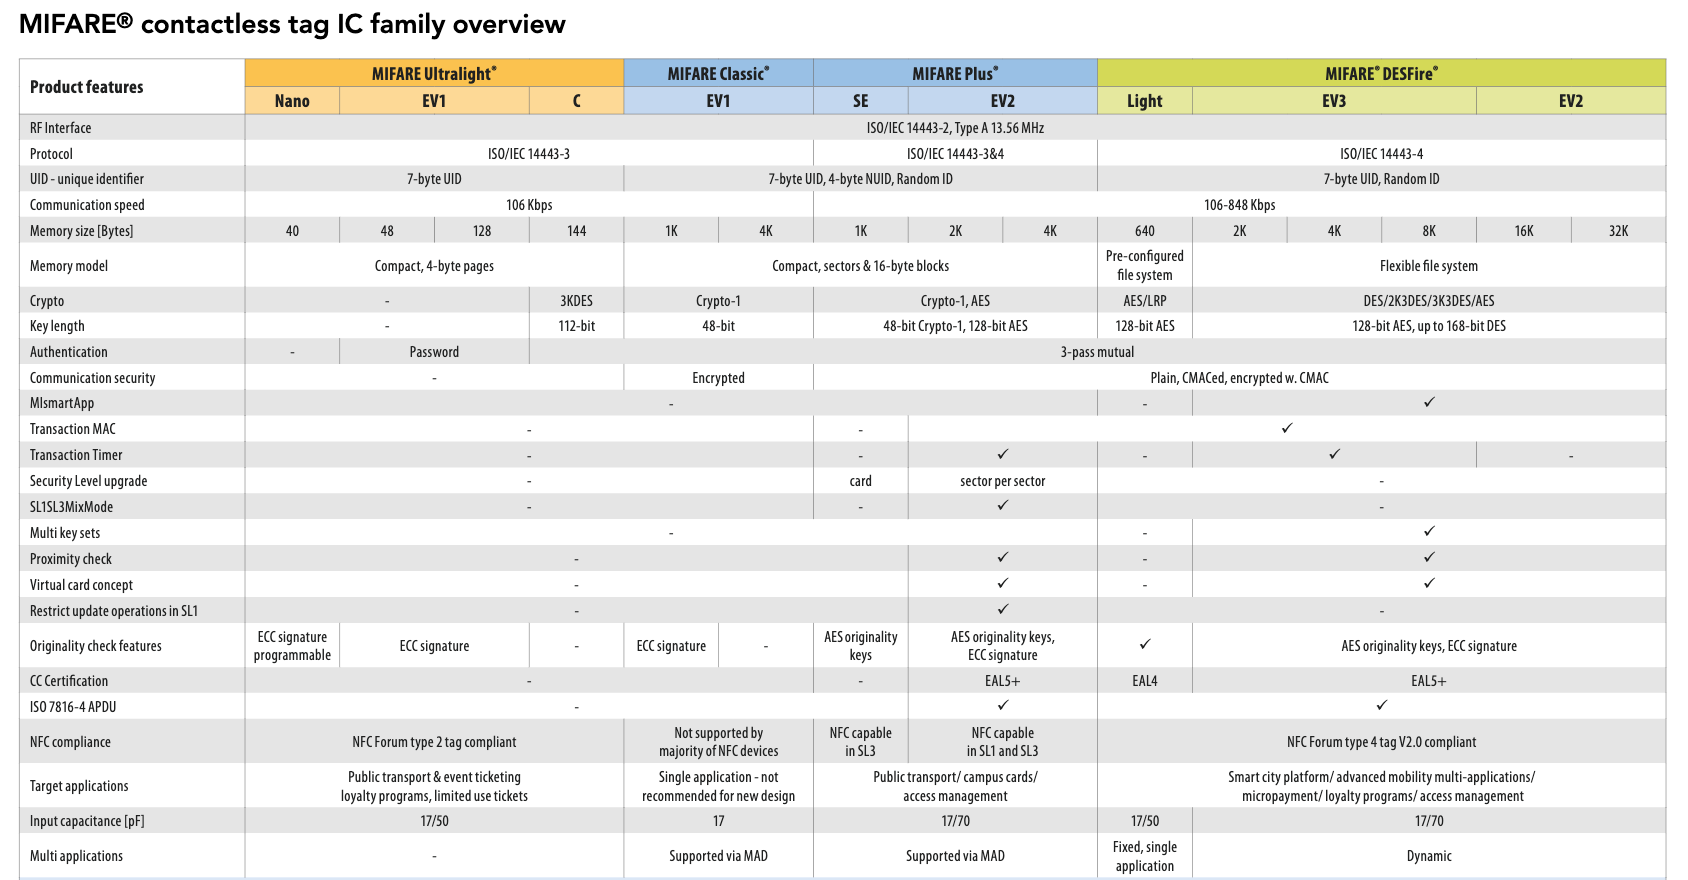
\includegraphics[width=1\textwidth]{gfx/mifare.png}}
	\caption{Mifareproduktfamilie}
	\label{fig:mifare}
\end{figure}

\section{Sender-Empfänger-System mit RFID}
\label{sec:theorie:rfid}
Im vorherigen Kapitel \ref{sec:theorie:mifare} wurden die Grundlagen und Vorteilen der MIFARE-Technologie für Smartcards erklärt. Im aktuellen Kapitel wird über die  Sender-Empfänger-System mit RFID beschrieben. Für die Implementierung der Aufgabe wird sowohl MIFARE-Smartcards als auch RFID-Tag-Mikrochips verwendet. Der letzte wird zum Identifizierung der auszuleihenden Raspi-Boards benutzt und auf der Rückseite des jeden Boards unter dem Schutzschirm geklebt werden. Beide Typs können mit dem RFID-Leser ACR122U-A9 von Advanced Card Systems abgelesen werden. Ab hier wird weiter nur den Begriff "Tag" sowohl für MIFARE-Smartcards als auch für RFID-Tag-Mikrochips verwendet und den Unterschied in Namen nicht weiter angemerkt. Die gespeicherte Daten warten darauf, gelesen zu werden. Die Antenne des Tags erhält Energie von einer RFID-Leseantenne. Mit der Stromversorgung der internen Batterie oder des Lesegeräts sendet das Tag Funkwellen an das Lesegerät zurück. Der Leser nimmt die Funkwellen des Tags auf und interpretiert die Frequenzen als Daten. RFID-Tags, die über einen Teil des elektromagnetischen Spektrums gesendet werden, und die genaue Frequenz können ausgewählt werden, um Interferenzen mit anderen elektronischen Geräten zu vermeiden. Der Leser sendet ein Signal an das Tag und liest seine Antwort \cite{website:13}. Der Leser verfügt über einen Funkempfänger, der als Transceiver bezeichnet wird und ein codiertes Funksignal an das Tag sendet. Das Signal aktiviert das Tag und der Transponder wandelt das Signal dann in eine nutzbaren Leistung um und sendet auf den Leser. Das Tag empfängt die Nachricht und antwortet dann mit seiner Identifikation und anderen Daten. Dies kann eine eindeutige Seriennummer des Produkts oder produktbezogene Daten sein. In der Abschlussarbeit wird nach der UID des Tags gefragt. 

\begin{wrapfigure}{l}{0.45\textwidth}
	\fbox{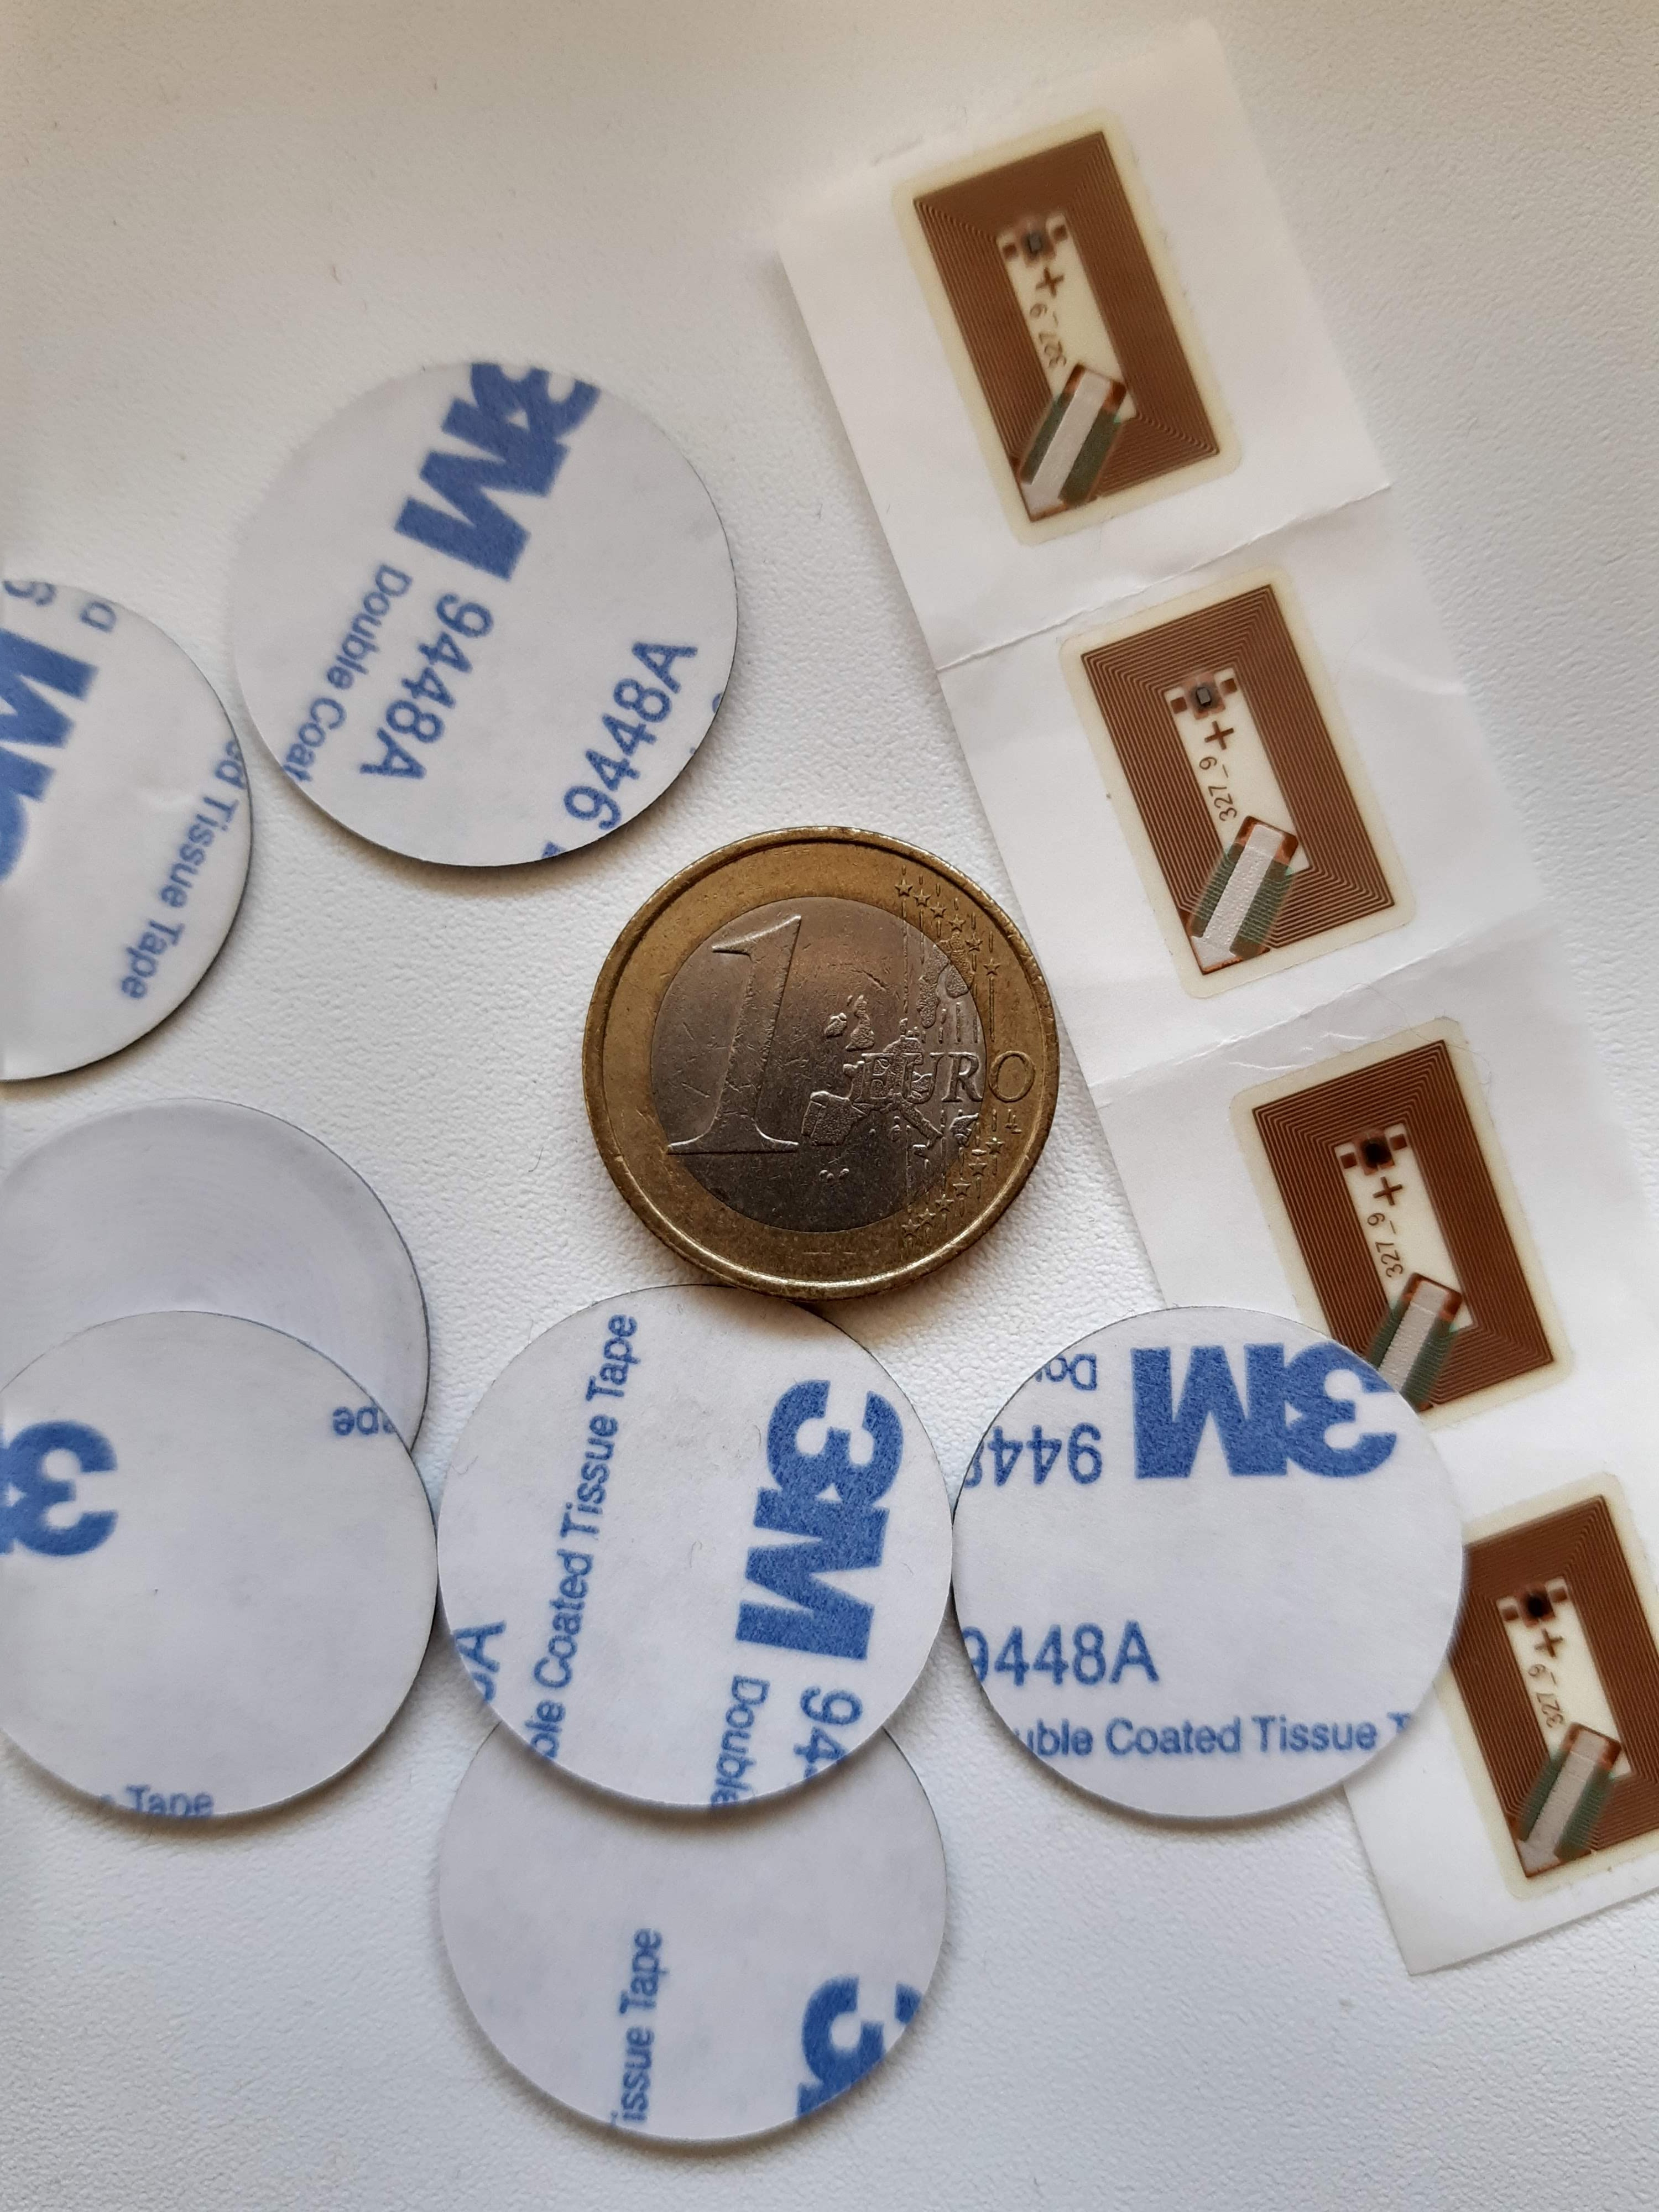
\includegraphics[width=0.42\textwidth]{gfx/tags.jpg}}
	\caption{Verschiedenen RFID-Tags}
	\label{fig:tags}
\end{wrapfigure}
Während sich jedes Sender-Empfänger-System mit RFID hinsichtlich Gerätetyp und Komplexität unterscheidet, enthält jedoch jedes RFID-System mindestens die folgenden vier Komponenten: Leser, Antennen, Tags und Kabel. Das einfachste System kann aus einem mobilen Hand-RFID-Lesegerät (mit integrierter Antenne) und RFID-Tags bestehen, während komplexere Systeme mit Multi-Port-Lesegeräten, GPIO-Boxen, zusätzlichen Funktionsgeräten, mehreren Antennen, Kabeln und RFID-Tags ausgelegt sind und ein komplettes Software-Setup benötigen können. RFID-Tag-Typ Bestimmt das RFID-System. Derzeit gibt es drei verschiedene Arten von Tags: \textbf{aktiv, semi-passiv und passiv}. Ein aktives Tag sendet mit seiner Batterie Radiowellen an einen Leser, während eine semi-passive Tag-Batterie in Gegenwart eines Lesers aktiviert wird. Aktive und semi-passive Tags werden über größere Entfernungen gelesen. Sie senden hohe Frequenzen von 850 bis 950 MHz, die von 30 Meter oder mehr gelesen werden können. Zusätzliche Batterien können die Reichweite eines Tags auf über 90 Meter erhöhen. Passive RFID-Tags haben keine Batterie und verwenden die vom Lesegerät übertragene Funkenergie als Stromquelle. Diese Tags werden bis zu ein paar Meter entfernt gelesen und sind kostengünstiger \cite{website:13}. Für die Markierung der Raspi-Boards im PSE-Labor werden die passive RFID-Tags verwendet, die für vorgesehenen Zwecken ideal dienen. Die runde benutzte im Abschlussprojekt RFID-Tags sind auf der Abbildung \ref{fig:tags} im Vergleich in der Große zu 1-Euro Münze zu sehen. RFID-Systeme können nach Tag- und Lesertyp klassifiziert werden: passiver Leser - aktiver Tag (PRAT), aktiver Leser - passiver Tag (ARPT) und aktiver Leser - aktiver Tag (ARAT). Das ARPT-System wird im PSE-Labor eingesetzt und verfügt über einen aktiven Leser und empfängt Authentifizierungssignalantworten von passiven Tags. Ich möchte an dieser Stelle auch noch anmerken, dass der Initialisierungsprozess für eine kontaktlose Karte viel komplizierter als für eine Kontaktkarte ist. Das meiste davon wird vom sogenannten Antikollisionszyklus besetzt. Eine Kollision tritt auf, wenn mehr als eine Karte gleichzeitig auf das elektromagnetische Feld der RFID-Leser trifft und der diese Karten voneinander unterscheiden muss. Der Algorithmus dieses Prozesses ist sehr komplex und umfasst mehrere zehn Seiten Beschreibung in den Normen ISO/IEC 14443-2 und ISO / IEC 14443-3. Daher werde ich ihn hier nicht angeben, da es nicht von Entwickler wirklich etwas zu machen benötigt wird - das Terminal und der RFID-Leser sind voll damit beschäftigt.

\section{Django Framework}
\label{sec:theorie:about_django}
Django ist ein Open Source-Webentwicklungsframework, das in der Python-Sprache geschrieben ist. Es wurde entwickelt, um so viele Prozesse wie möglich zu automatisieren, sodass es sich auf die Softwareentwicklung konzentriert werden können, ohne Zeit mit dem Einrichten des Servers verschwenden zu müssen. Django wurde ursprünglich so konzipiert, dass es lose Kopplung zwischen verschiedenen Teilen der Infrastruktur hat, sodass es unabhängig voneinander gearbeitet werden kann. Diese Unabhängigkeit bedeutet, dass es in der Entwicklungsprozess nur die Teile von Django verwendet werden kann, die benötigt werden, ohne sich um Probleme mit der Interdependenz von Komponenten kümmern zu müssen. Durch die Verwendung von Django wird die erforderliche Codemenge reduziert, wodurch das Schreiben von Webanwendungen schneller und die Wartung Ihrer Anwendung in Zukunft erheblich vereinfacht wird. Django folgt strikt dem DRY-Prinzip (Don't Repeat Yourself), dass jeder einzelne Code oder jede einzelne Daten an nur einem Ort gespeichert werden sollte. Dies vereinfacht und beschleunigt den Softwareänderungsprozess erheblich, da eine Anwendung, die geändert werden muss, an einem einzigen Ort ausgeführt werden muss.

Nach der Django Instalation und dem Erstellen eines Projekts ist es nützlich, die erstellte Projektstruktur zu betrachten \cite{website:16}:

\begin{itemize}
	\item \textbf{manage.py} ist ein Befehlszeilenprogramm, mit dem auf verschiedene Weise mit  Django-Projekt interagiert wird . Diese Datei muss nicht geändert werden.
	
	\item \textbf{acaLoanRaspiBoard} Projektarbeitsverzeichnis enthält:
	\subitem \textbf{$\_\_init\_\_.py$}: Eine leere Datei, die Python mitteilt, dass dieses Verzeichnis für das Python-Paket bestimmt ist.
	\subitem \textbf{$settings.py$}: Die Einstellungen und Konfigurationsdatei für das Django-Projekt.
	\subitem \textbf{$urls.py$}: Die URL-Beschreibungsdatei für dieses Django-Projekt.
	\subitem \textbf{$asgi.py$}: Damit kann die Anwendung mit einem Webserver unter Verwendung des ASGI-Protokolls arbeiten.
\end{itemize}
Die generierte Datei settings.py enthält eine Grundkonfiguration für die Verwendung einer SQLite-Datenbank und eine Liste von Django-Anwendungen, die standardmäßig zum Projekt hinzugefügt werden sollen. In der Datei settings.py ist es möglich, den Debug-Modus des Projekts zu aktivieren / deaktivieren. Wenn "Debug=true" festgelegt ist, zeigt der Server  bei Auftreten einer nicht erfassten Ausnahme detaillierte Fehlermeldung an. Es muss beim Wechsel zur Produktionsversion auf "false" gesetzt, da mit aktiviertem Debugging alle Benutzer vertrauliche Projektdaten sehen können. 

Die Architektur von Django basiert auf den Ideen des The Model-View-Controller (MVC) Design Pattern, womit Anwendungsschicht, Benutzeroberfläche (UI) und Datenzugriffsebenen getrennt werden, sodass jede dieser Ebenen unabhängig von anderen geändert werden kann. Als Konzept ist das MVC-Entwurfsmuster wirklich einfach zu verstehen \cite[pp. 15-16]{george:django}:
\begin{itemize}
	\item \textbf{Das Modell (M)} ist ein Modell oder eine Darstellung Ihrer Daten. Es handelt sich nicht um die tatsächlichen Daten, sondern um eine Schnittstelle zu den Daten. Mit dem Modell können Sie Daten aus Ihrer Datenbank abrufen, ohne die Feinheiten der zugrunde liegenden Datenbank zu kennen. Das Modell stellt normalerweise auch eine Abstraktionsschicht mit Ihrer Datenbank bereit, sodass Sie dasselbe Modell mit mehreren Datenbanken verwenden können.
	\item \textbf{Die Ansicht (V)} ist das, was mit den Augen gesehen werden kann. Dies ist die Präsentationsebene für das Modell. Auf dem Computer wird die Ansicht im Browser für eine Web-App oder in der Benutzeroberfläche für eine Desktop-App angezeigt. Die Ansicht bietet auch eine Schnittstelle zum Sammeln von Benutzereingaben.
	\item \textbf{Der Controller (C)} steuert den Informationsfluss zwischen dem Modell und der Ansicht. Mithilfe der programmierten Logik wird entschieden, welche Informationen über das Modell aus der Datenbank abgerufen und welche Informationen an die Ansicht übergeben werden. Es erhält auch Informationen vom Benutzer über die Ansicht und implementiert die Aufgaben der Anwendung: entweder durch Ändern der Ansicht oder durch Ändern von Daten über das Modell oder durch Ändern die beiden Elementen.
\end{itemize}

\section{Grundlagen der Webanwendungen}
\label{sec:theorie:webapp}
In diesem Kapitel werden die grundlegenden Begriffe zum Entwerfen und Erstellen eines Webanwendung erläutert. Hierbei konzentrieren wir uns auf die Probleme im Zusammenhang mit der Verarbeitung von HTTP-Anfragen und -Antworten (siehe Kapitel \ref{sec:theorie:api}). Da in den letzten Jahren sich Webanwendungen rasant weiterentwickelt und die Desktop-Lösungen schrittweise ersetzt haben, es sollte auch nicht unerwähnt bleiben, welche Vorteile die Webanwendungen haben:
\begin{itemize}
	\item \textbf{Zugriff von jedem Gerät} Die Webanwendung kann überall auf der Welt von einem Computer, Tablet oder Smartphone zugegriffen und verwendet werden. Notwendig ist, dass dem Gerät eine Internetverbindung zur Verfügung steht.
	
	\item \textbf{die Kostenersparnis} Webanwendungen können auf allen Plattformen ausgeführt werden und müssen nicht mehr separat für Android und iOS entwickelt werden.
	
	\item \textbf{Anpassungsfähigkeit} Wenn native Anwendungen bestimmte Betriebssysteme erfordern, jedoch können jedes Betriebssystem (Windows, MAC, Linux usw.) und jeder Browser (Internet Explorer, Opera, FireFox, Google Chrome usw.) für die Arbeit mit einer Webanwendung. ) verwendet werden.
	
	\item \textbf{Keine Software zum Herunterladen} Es ist günstig und einfach dem Endnutzer zu liefern, zu warten und zu aktualisieren. Das Aktualisieren auf die neueste Version erfolgt beim nächsten Laden der Webseite.
	
	\item \textbf{Netzwerksicherheit} Das Websystem verfügt über einen einzigen Einstiegspunkt, der zentral geschützt und konfiguriert werden kann.
	
	\item \textbf{Skalierbarkeit} Mit zunehmender Belastung des Systems ist es nicht erforderlich, die Leistung des Computer von Endbenutzer zu erhöhen. Mit einer Webanwendung kann in der Regel nur mithilfe von Hardwareressourcen eine größere Datenmenge verarbeitet werden, ohne den Quellcode neu zu schreiben und die Architektur ändern zu müssen.
	
	\item \textbf{Verhinderung von Datenverlust} Benutzerdaten werden in der "Cloud" gespeichert, für deren Integrität die Hosting-Anbieter verantwortlich sind, deswegen vom Verlust geschützt, falls die Festplatte des Computers beschädigt wird.
\end{itemize}

Ich möchte an dieser Stelle auch noch ein Konzept des Caches erklären, bei dem häufig verwendete Daten, anstatt jedes Mal aus der Datenbank abgerufen, berechnet oder auf andere Weise vorbereitet, an einem schnell zugänglichen Ort gespeichert werden. Zum Beispiel erhielt Django eine Anfrage, Daten für ein Diagramm in einem Bericht abzurufen. Daten aus der Datenbank werden abgeholt, vorbereitet und abgelegt in einer Datenbank mit schnellem Zugriff z.B. "memcached", die beispielsweise für eine Stunde zwischengespeichert wird. Bei der nächsten Anfrage werden die notwendigen Daten sofort von "memcached" erhalten und an das Frontend gesendet. Wenn es festgestellt wird, dass die Daten nicht mehr relevant sind, werden sie ungültig beziehungsweise gelöscht aus dem Cache.

\subsection{Client-Server Kommunikation}
\label{sec:theorie:http}
Als nächstes geht die Frage nach, wie Client und Server miteinander kommunizieren können. Der Client spricht mit dem Server über \hyperref[sec:appendix:http]{das HTTP-Protokoll}. Das HTTP-Protokoll setzt die Verwendung einer Client-Server-Datenübertragungsstruktur voraus. Es verwendet normalerweise Port 80 und as Transportschichtprotokoll - TCP. Das HTTP-Protokoll ist in RFC 1945 (HTTP 1.0 \cite{website:httprfc1945}), 2068 \cite{website:httprfc2068} und 2616 (HTTP 1.1) definiert. Die Clientanwendung generiert eine Anforderung und sendet sie an den Server. Anschließend verarbeitet die Serversoftware diese Anforderung, generiert eine Antwort und sendet sie an den Client zurück \cite[pp.33-34]{shklar:webapplication}. Die Clientanwendung kann dann weiterhin andere Anforderungen senden, die auf ähnliche Weise behandelt werden. Wenn ein Webserver eine Anforderung zum Bereitstellen einer statischen Webseite erhält, sendet er die Seite direkt an den Browser.\cite{website:2} Wenn jedoch eine dynamische Seite angefordert wird, sind die Handlungsweise des Webservers nicht so einfach. Der Server übergibt die Seite an ein spezielles Programm, das die letzte Seite bildet. Ein solches Programm wird als Anwendungsserver bezeichnet. Der Anwendungsserver liest den Code auf der Seite, rendert die letzte Seite gemäß dem gelesenen Code und entfernt sie dann von der Seite. Als Ergebnis all dieser Operationen wird eine statische Seite erhalten, die an den Webserver übertragen wird, der sie wiederum an den Client-Browser sendet. Alle Seiten, die der Browser empfängt, enthalten nur HTML-Code \cite{website:2}. 
 
\begin{figure}[h!]
	\centering
	\fbox{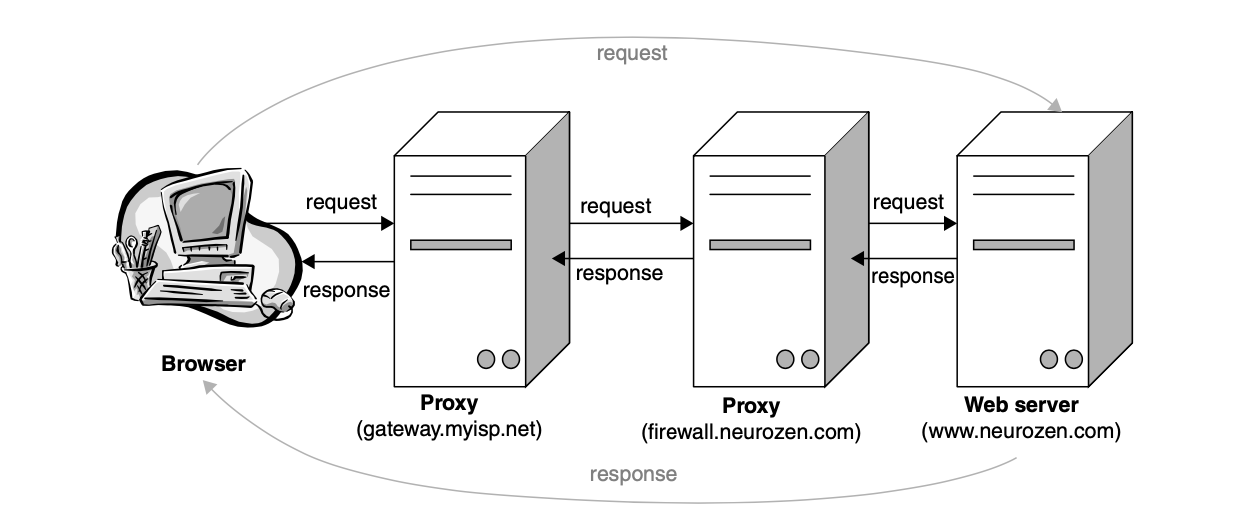
\includegraphics[width=1\textwidth]{gfx/req_res.png}}
	\caption{Die virtuelle Anforderungs- / Antwortschaltung}
	\label{fig:http_req}
\end{figure}

Dieses grundlegende Paar Anforderung-Antwort wird im nächsten Kapitel \ref{sec:theorie:api} untersucht. In der Praxis kommunizieren Server und Browser selten direkt - dazwischen befinden sich ein oder mehrere Proxys. Eine Verbindung ist als virtuelle Verbindung definiert, die aus HTTP-Agenten besteht, einschließlich des Browsers, des Servers und der am Austausch teilnehmenden Zwischenproxys (Abbildung \ref{fig:http_req} \cite[pp.33-34]{shklar:webapplication}).


HTTP definiert eine Reihe von Anforderungsmethoden, um die gewünschte Aktion anzugeben, die für eine bestimmte Ressource ausgeführt werden soll. Sie werden als HTTP-Verben bezeichnet.
Diese Anforderungsmethoden sind unten aufgeführt:
\begin{itemize}
	\item \textbf{GET} ist die einfachste Anforderungsmethode. Wenn eine URL in Browser eingeben oder auf einen Hyperlink geklickt wird, um eine andere Seite zu besuchen, verwendet der Browser die GET-Methode, um die Anforderung an den Webserver zu senden.
	\item \textbf{POST} wird benutzt, um eine neue Ressource zu erstellen. POST-Anforderungen enthalten normalerweise Daten zum Erstellen einer neuen Ressource.
	\item \textbf{PUT} ist zum Aktualisieren einer vorhandenen Ressource. Der Inhalt kann aktualisierte Daten für die Ressource enthalten.
	\item \textbf{DELETE} ist zum Löschen einer vorhandenen Ressource.
\end{itemize}

\subsection{Grundlagen der REST API}
\label{sec:theorie:api}
In der Client-Server-Kommunikation haben wir zunächst zwei Partner: den Client und den Server. Um die Kommunikation zwischen diesen beiden Partnern zu verstehen, müssen wir einige einfache Themen kennen:
\begin{itemize}
\item \textbf{Anforderungen} werden vom Client gesendet, um den Server nach Daten wie Dateien zu fragen oder den Server über Ereignisse zu informieren, z. B. dass sich ein Benutzer mit seinen Anmeldeinformationen anmelden möchte
\item \textbf{Antwort} wird vom Server an den Client gesendet und ist die Reaktion des Servers auf eine Anforderung des Clients. 
\end{itemize}

Die ankommenden Anforderungen muss vom Server interpretiert und weitergeleitet werden. Während dieses Schritts übernimmt der Webserver die Verantwortung für Bestimmung, welche Maßnahmen zur Verarbeitung der Anforderung erforderlich sind. Diese Aktion kann das einfache Abrufen einer statischen HTML-Datei oder der Zugruf zur Datenbank sein. Das kann komplexe Funktionen ausführen, die mit einer vollständigen Webanwendung verbunden sind \cite[p.204]{shklar:webapplication}. Wenn ein Benutzer versucht, auf eine Webanwendung zuzugreifen, sendet der Browser zuerst eine HTTP-Anforderung an einen Webserver. Die mit der Anforderung verknüpften Informationen (häufig als Anforderungskontext bezeichnet) umfasst die weitere Informationen, die in der URL, dem Anforderungsheadern und dem Nachrichtentext enthalten sind. Es enthält auch Sitzungsinformationen, die den Anwendungsstatus über aufeinanderfolgende Anforderungen hinweg beibehalten \cite[p.205]{shklar:webapplication}.

Die Client-Server-Kommunikation ist zustandslos. Dies bedeutet, dass sich der Server keine Informationen über den Status des Clients merken muss, während der Client alle Informationen in seine Anforderung aufnehmen muss.

Das REST- oder RESTful-API-Design (Representational State Transfer) ist eine Client-Server-Architektur und nutzt normalerweise HTTP-Protokoll \cite{website:rest}. Der Server speichert und bearbeitet Informationen und stellt sie dem Benutzer auf effiziente Weise zur Verfügung. Der Client nimmt diese Informationen und zeigt sie dem Benutzer an und verwendet sie, um nachfolgende Informationsanforderungen auszuführen. Diese Trennung von Funktionsweise ermöglicht es sowohl dem Client als auch dem Server, sich unabhängig voneinander zu existieren und entwickelt werden, da nur die Kommunikationsschnittstelle gleich bleiben muss  \cite{website:rest2}. In einem REST-API-Aufruf werden eine Teilmenge der HTTP-Methoden für die Aktionen verwendet, die wir ausführen müssen. Diese Methoden wurden oben im Kapitel \ref{sec:theorie:http} schon erklärt. REST-APIs geben normalerweise die von Benutzter angeforderten Daten im JSON-Format zurück, dessen Payload eine String (Zeichenfolge) ist. Bevor die Daten tatsächlich verwendet werden können, müssen diese Zeichenfolge analysiert und in Objekte umgewandelt werden. Die Funktionsweise das REST-APIs von acaLoan-System sind in Kapitel \ref{sec:display_client:protokoll} nachzulesen.

\subsection{Clientseitiges JavaScript}
\label{sec:theorie:js}
Das Document Object Model (DOM) ist eine Programmierschnittstelle für HTML- und XML-Dokumente. Es stellt die Seite dar, sodass Programme die Dokumentstruktur, den Stil und den Inhalt ändern können \cite{website:dom}. Clientseitiges JavaScript (CSJS) ermöglicht die Verbesserung und Bearbeitung von Webseiten über den soforten Zugang zu den Knoten des DOM: in einer Browserumgebung hat Ihr Code Zugriff auf Dinge, die nur vom Browser bereitgestellt werden, wie das Dokumentobjekt für die aktuelle Seite, das Fenster, Funktionen wie Warnungen, die eine Nachricht anzeigen usw. Die Hauptaufgaben von clientseitigem JavaScript sind die Validierung von Eingabe, Animation, Bearbeitung von UI-Elementen, Anwenden von Stilen und einige kleine Berechnungen können durchgeführt werden. Bei der Webentwicklung ist es der Browser auf dem Computer des Benutzers, der diesen Javascript Code ausgeführt \cite{website:csjs}. Bei der Implementierung der Aufgabestellung für acaLoan-Systen wird davon ausgegangen, dass der Chrome-Browser als Rendering-Frontend verwendet wird, dies ist jedoch nicht streng Anforderung und der Client sollte ohne Probleme mit anderen modernen Browsern arbeiten, da der Code des clientseitigen JavaScripts in einer Mehrheit von Browsern ausgeführt werden kann. 

Ein wichtiges Merkmal von JavaScript ist die Möglichkeit, Ereignishandler (event handlers) zu definieren - beliebige Codeteile, die ausgeführt werden, wenn ein bestimmtes Ereignis auftritt. Normalerweise werden diese Ereignisse vom Benutzer ausgelöst, wenn er beispielsweise die Maus über einen Hypertext-Link bewegt, einen Wert in ein Formular eingibt oder in einem Formular auf die Taste Senden klickt. Diese Funktion zur Ereignisbehandlung hat eine wichtigste Bedeutung, da für die Programmierung mit grafischen Oberflächen wie HTML-Formularen ein ereignisgesteuertes Modell erforderlich ist. JavaScript kann jede Art von Aktion als Reaktion auf Benutzerereignisse auslösen. Typische Beispiele könnten sein, eine spezielle Nachricht in der Statuszeile anzuzeigen, wenn der Benutzer die Taste drückt.  Sodass wird es im acaLoan-System nach dem Drücken die Taste "Loan / Return Board" und erfolgreichen Ablesen der Studentenkarte den Name der Studierende und die Nummer des schon zugewiesenen Boards angezeigt.

In diesem Kapitel wurden die Grundlagen der Webanwendungen erklärt, die als Überblick zum Verstehen der zukünftigen Verwendung der entwickelte Software im PSE-Labor dienen sollten.
